\chapter{Results}
\label{ch:results}

% sections
% 1 qualitative analysis (added by me)
% 2 setup
% 3 acquisition params
% 4 data treatment



% intro to results
This chapter presents the results of the thesis.
The results are divided into four parts: qualitative analysis of the spectra, characterization of the setup, optimization of the acquisition parameters, and data treatment.
As seen in the SE images presented in \cref{method:SE_images}, the areas chosen for the analysis are homogeneous and relatively clean.
Scratched areas on the GaSb specimen are shown in \cref{fig:SE_images:GaSb} panel (b), where some spectra were acquired, but not included in the results of this thesis.
% TODO discuss: the scratched areas behaved as expected, yielding poorer results than the homogeneous areas. ISO etc.



% 1 qualitative analysis
\section{Qualitative analysis}
\label{results:qualitative_analysis}

Here, an overview of the spectra is presented, where some characteristics and artifacts are identified, before addressing the setup parameters in \cref{results:setup}, acquisition parameters in \cref{results:acquisition_parameters}, and quantification results in \cref{results:quantitative}.
General plots of the spectra are given in \cref{fig:results:overviewGaSb_withArtifacts,fig:results:GaSb_voltages,fig:results:GaAs_voltages}.



% figures/results/spectrum_overview.pdf
\begin{figure}[hbtp]
    \centering
    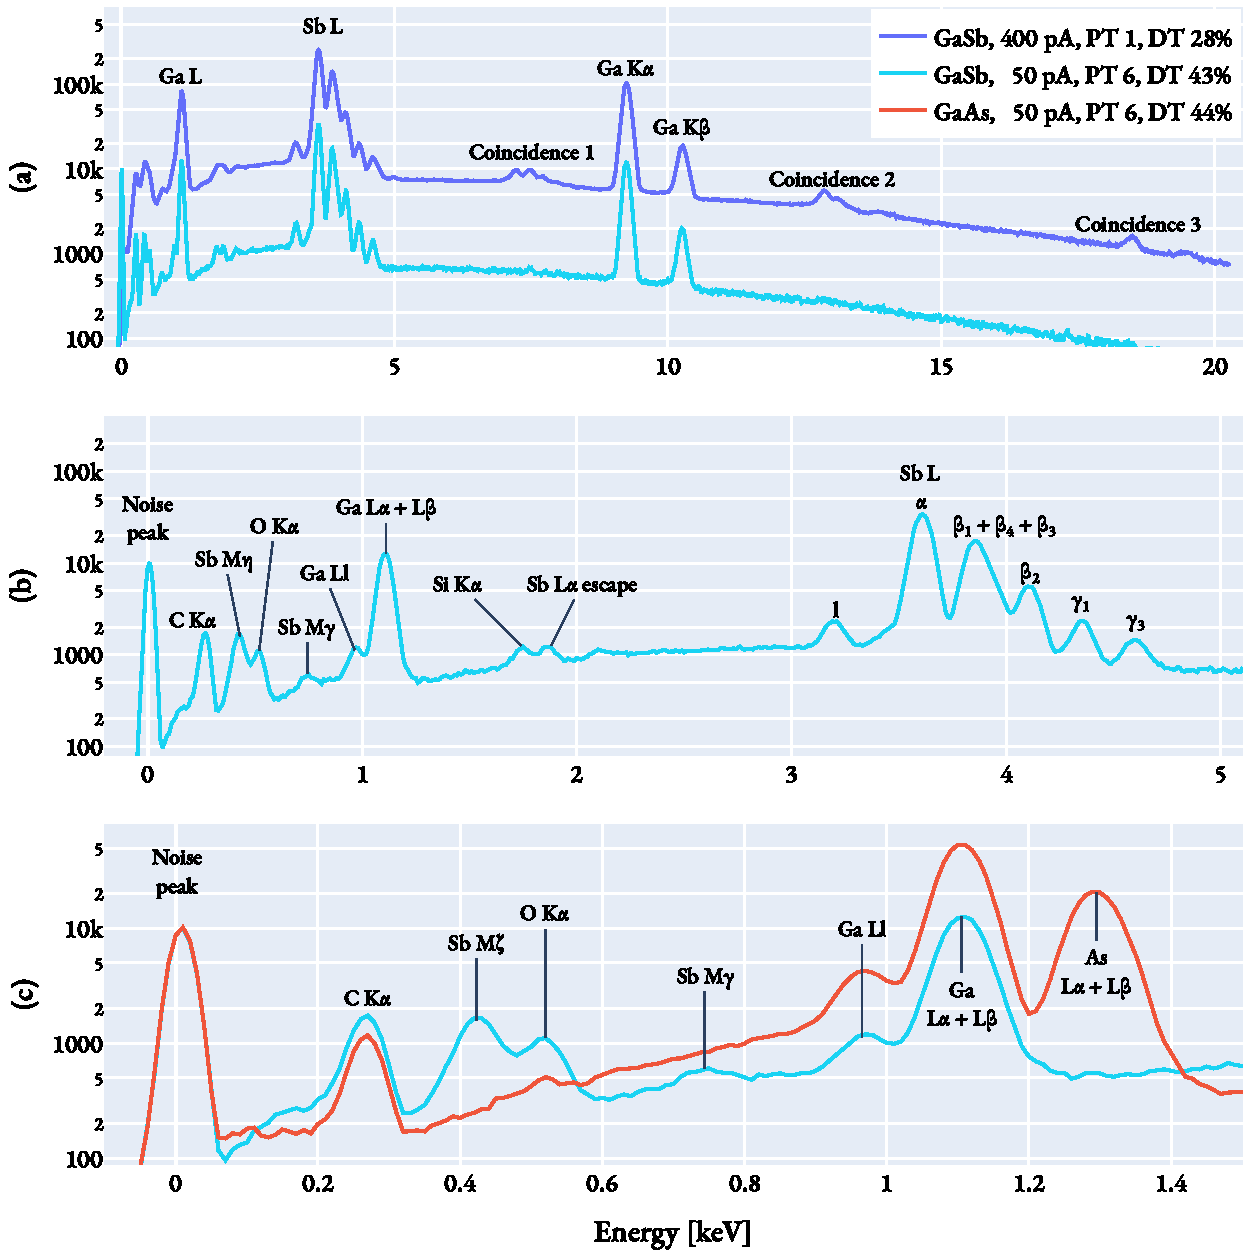
\includegraphics[width=0.99\linewidth]{figures/results/spectrum_overviews.pdf}
    \caption{
        Overview of the GaSb spectra.
        The blue line in panel (a) have lower resolution and more artifacts than the light blue line.
        The light blue line is plotted in panel (b) over a shorter energy range, and with peaks annotated.
        Panel (c) show the light blue line on an even shorter energy range, with the GaAs spectrum in red for reference.
        All three spectra are acquired with 30 kV.
    }
    \label{fig:results:overviewGaSb_withArtifacts}
\end{figure}


% figures/results/GaAs_voltages.pdf
\begin{figure}[hbtp]
    \centering
    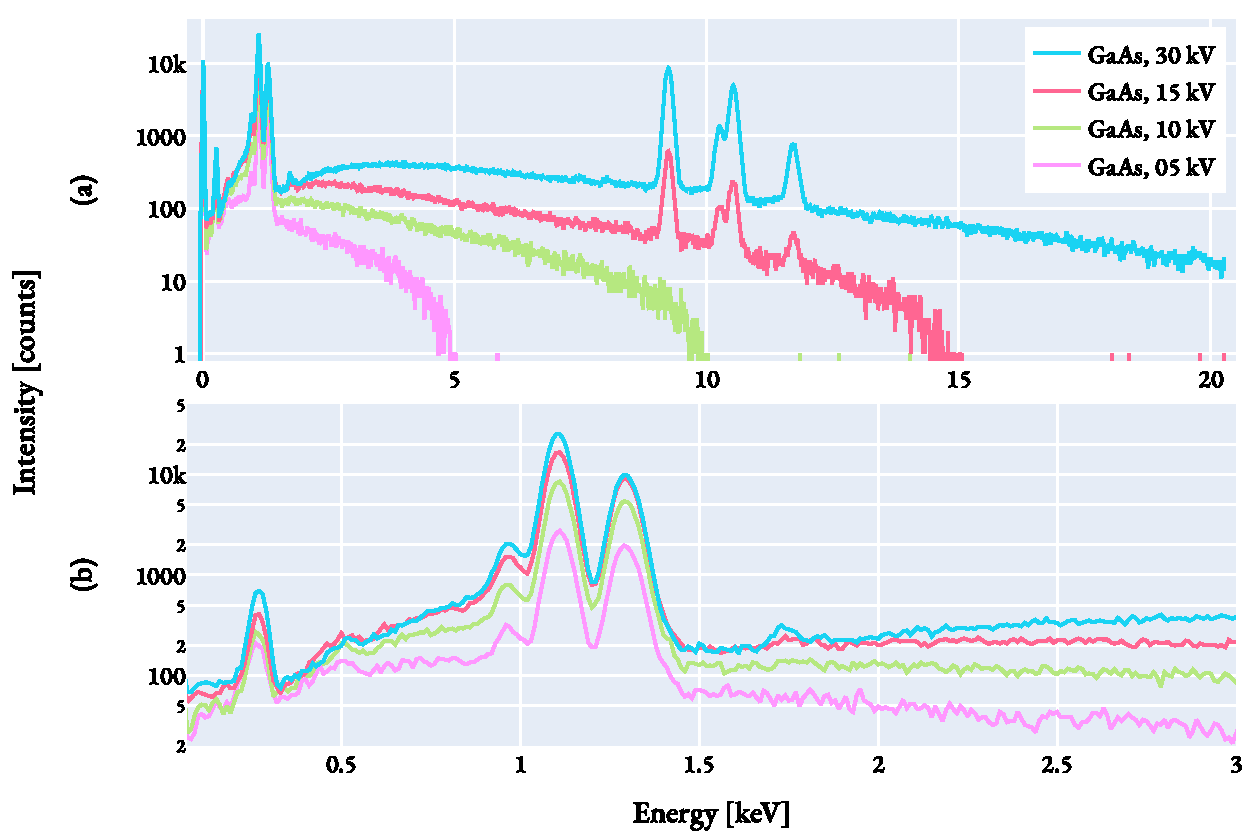
\includegraphics[width=0.85\linewidth]{figures/results/GaAs_voltages.pdf}
    \caption{
        Group (A), the GaAs voltage series.
        The figure gives an overview of the spectra, and show the effect of overvoltage.
        All four spectra have $i_b$ = 25 pA and PT 6.
    }
    \label{fig:results:GaAs_voltages}
\end{figure}


% figures/results/GaSb_voltages.pdf
\begin{figure}[hbtp]
    \centering
    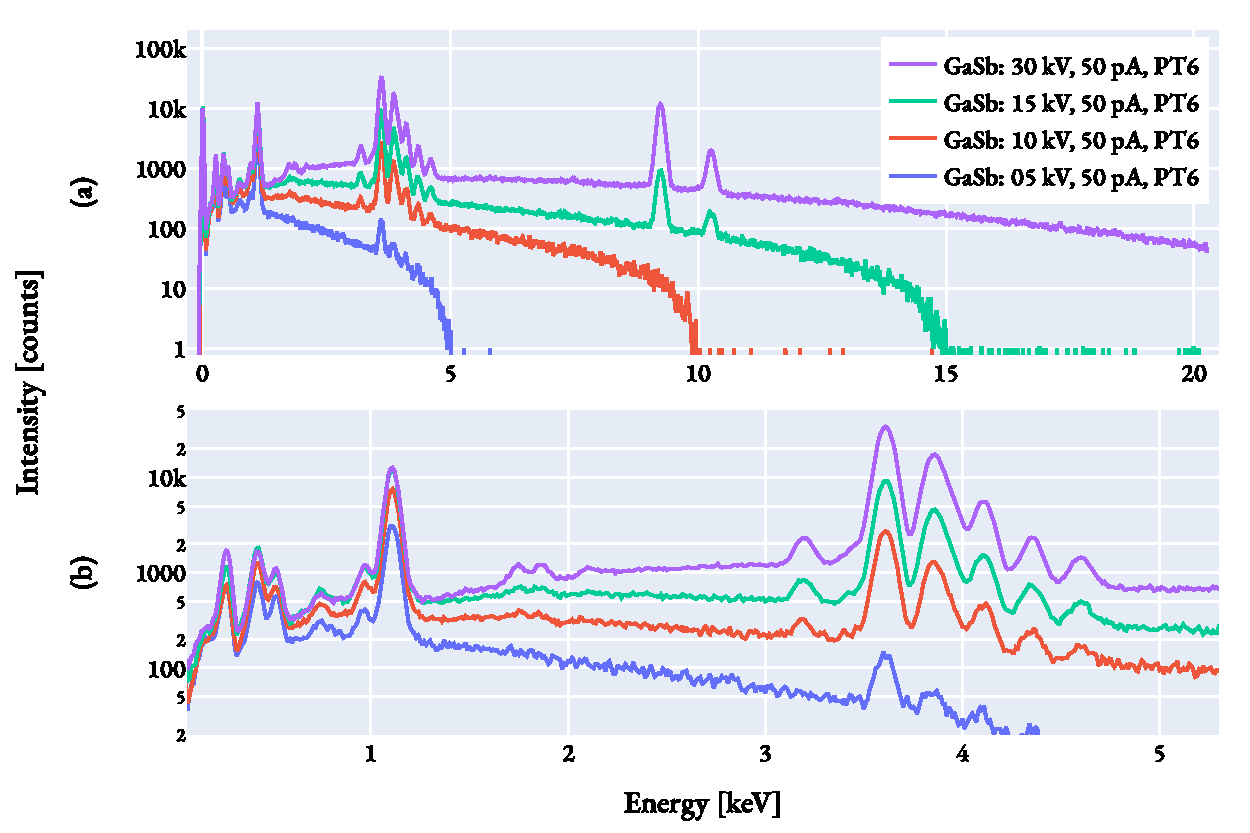
\includegraphics[width=0.85\linewidth]{figures/results/GaSb_voltages.pdf}
    \caption{
        Group (B), the GaSb voltage series.
        The figure serves the same purpose as \cref{fig:results:GaAs_voltages}, but for GaSb.
        % Additionally, an increased amound of coincidence counts compared to the GaAs spectra is visible in the tailing backgrounds, especially at 15 kV.
        The tailing background is the vertical lines above $E_0$.
        All four spectra have $i_b$ = 50 pA and PT 6.
    }
    \label{fig:results:GaSb_voltages}
\end{figure}





% \subsection*{Lines}
% \label{results:qualitative_analysis:lines}

The lines given in \cref{tab:theory:lineEnergies} for Ga, As, and Sb have been identified in the spectra.
All spectra also had a peak at C K$\alpha$.
% TODO Ton: discus this C_Ka artifact, origin, in discussions
% TODO Ton: No other common peaks like Fe, or Si from set-up?
The GaSb spectra included a well-defined O K$\alpha$ peak, while the GaAs spectra had barely any signal from the O K$\alpha$ line.
% TODO discuss: the O Ka peak might also be a Sb M-line, but I have not found the energy of the Sb M-lines.
As annotated in \cref{fig:results:overviewGaSb_withArtifacts}, the GaSb spectra also included two Sb M-signals: $\eta$ and $\gamma$, where $\eta$ is a clearly defined peak, while $\gamma$ is a slight increase in intensity.
These two M-peaks are not listed in the HyperSpy database, but were found through AZtec \cite{aztec_manual} and other literature \cite{liao2006practical}.
% TODO discuss: M lines are present in the absorption plot of GaSb



% \subsection*{Artifacts}
% \label{results:qualitative_analysis:artifacts}

Artifacts are present in all spectra, in varying degrees.
The artifacts identified are listed and described in \cref{tab:results:artifacts}.
The artifacts present in the spectra are the background, the noise peak, the carbon and oxygen stray peak, coincidence peaks, the internal Si fluorescence peak, and the Si escape peak from Sb La.

% The background is present in all spectra, and with increasing background intensity with higher count rates.
% The effect of a strong absorption edge which reduce the background intensity above its energy is most prominent in the GaAs spectra.
% Here it is the absorption edge in the L-peaks which reduce the background intensity abruptly above the L-peaks.
% Coincidence peaks are only present in some spectra, and are most prominent in the spectra with very high count rates.
% The spectra with beam energy 5, 10, and 15 keV also show coincidence events above $E_0$, e.g. visible in panel (a) in \cref{fig:results:GaSb_voltages}.


\begin{table}[phtb]
	\begin{center}
		\caption{
			The artifacts present in the spectra.
			See \cref{fig:results:overviewGaSb_withArtifacts,fig:results:GaSb_voltages,fig:results:GaAs_voltages}.
		}
		\renewcommand*{\arraystretch}{1.4}
		\label{tab:results:artifacts}
		\begin{tabular}{p{3.5cm}p{11.1cm}}
			\hline
			\textbf{Artifact}                                & \textbf{Where the articat is present and a comment}                                                                                                                                                                                                                                                                                                                                                                                             \\
			\hline
			Background                                       & All spectra. Increase with higher count rate.                                                                                                                                                                                                                                                                                                                                                                                                   \\
			Absorption edge effect on background             & Most prominent in GaAs. Reduces the background intensity above the Ga L absorption edge. In \cref{fig:results:GaAs_voltages} panel (b) the background drop from around 600 to around 170 counts.                                                                                                                                                                                                                                                \\
			Noise peak                                       & All spectra. Located almost at 0 keV.                                                                                                                                                                                                                                                                                                                                                                                                           \\
			Coincidence peaks                                & Only the spectra with very high count rates. \cref{fig:results:overviewGaSb_withArtifacts} with GaSb taken at 30 kV, 400 pA, and PT1 show coincidence peaks from: (Sb L + Sb L), (Sb L + Ga K), and (Ga K + Ga K).                                                                                                                                                                                                                              \\
			Tailing background noise from coincidence events & Present in spectra taken at 5, 10, and 15 kV. Coincidence events from two arbitrary counts give a tailing background. Exemplified by the green 15 kV line in \cref{fig:results:GaSb_voltages} panel (a), where vertical lines (one count each) are present between 15 and 20 keV.                                                                                                                                                               \\
			Internal fluorescence peak                       & Visible in some spectra. A low signal, barely a peak in some spectra, at Si K$\alpha$.                                                                                                                                                                                                                                                                                                                                                          \\
			Si escape peak                                   & Most GaSb spectra show some escape signal from Sb L$\alpha$ at 1.86 keV, labeled in \cref{fig:results:overviewGaSb_withArtifacts} panel (b). The coincidence counts from (Sb L + Sb L) marked as "Coincidence 1" in \cref{fig:results:overviewGaSb_withArtifacts} panel (a) has one peak at 7.2 keV and one at 7.5 keV, where the latter cound be a combination of coincidence events and escape counts from Ga K$\alpha$ (9.25 - 1.74 = 7.51). \\
			Stray C                                          & All spectra show a C K$\alpha$ peak, with some variation in intensity.                                                                                                                                                                                                                                                                                                                                                                          \\
			Stray O                                          & All spectra of GaSb show an O K$\alpha$ peak. The GaAs spectra have much lower, but still present signal at 0.52 keV.                                                                                                                                                                                                                                                                                                                           \\
			\hline
		\end{tabular}
	\end{center}
\end{table}



























% 2 setup
\section{Characterization of the setup}
\label{results:setup}

The parameters of the setup are: energy resolution, the energy scale and offset, peak ratios, and deviations in peak positions.
To show how the info in a single spectrum varies with the selected line of reference, information from the lines are presented from two selected spectra in \cref{tab:results:lines_info_30kV_50pA}.
The two selected spectra are both acquired with 30 kV, 50 pA, PT 6, DT 44\%, and ICR = 17k cps for GaSb and ICR = 16.5k cps for GaAs.
The table lists the theoretical energy of the line, the change in position after calibration, the FWHM of the peak, the area of the peak, the Fiori P/B of the line, and the estimated FWHM of Mn K$\alpha$ using \cref{eq:estimateFWHM}.


\begin{table}[phtb]
    \begin{center}
        \caption{
            Info from the lines acquired at 30 keV, 50 pA, and PT 6.
            The lines are sorted by area (counts in the peak).
            %The table lists the theoretical energy of the line, the change in position after calibration, the FWHM of the peak, the area of the peak, the Fiori P/B of the line, and the estimated FWHM of Mn K$\alpha$ using \cref{eq:estimateFWHM}.
            Both the GaAs and GaSb spectra have DT 44\%, with ICR = 17k cps for GaSb and ICR = 16.5k cps for GaAs.
        }
        \renewcommand*{\arraystretch}{1.4}
        \label{tab:results:lines_info_30kV_50pA}
        \begin{tabular}{llrlrrrp{2.5cm}}
            \hline
            \textbf{Specimen} & \textbf{Line} & \textbf{Energy} & \textbf{$\Delta$ E} & \textbf{FWHM} & \textbf{Area}     & \textbf{Fiori P/B} & \textbf{Estimated FWHM(Mn K$\alpha$)} \\
                              &               & \emph{[keV]}    & \emph{[eV]}         & \emph{[eV]}   & \emph{[k counts]} &                    & \emph{[eV]}                           \\
            \hline
                              & Ga L$\alpha$  & 1.098           & 2                   & 67            & 333               & 586                & 128                                   \\
                              & Ga K$\alpha$  & 9.252           & 2                   & 163           & 302               & 762                & 134                                   \\
                              & As K$\alpha$  & 10.544          & 2                   & 173           & 183               & 622                & 135                                   \\
            GaAs              & As L$\alpha$  & 1.282           & 2                   & 72            & 140               & 236                & 129                                   \\
                              & Ga L$\beta$   & 1.125           & 0                   & 68            & 56                & 97                 & 129                                   \\
                              & Ga K$\beta$   & 10.264          & 2                   & 161           & 39                & 124                & 123                                   \\
                              & As K$\beta$   & 11.726          & 2                   & 181           & 27                & 117                & 135                                   \\
                              & As L$\beta$   & 1.317           & 0                   & 71            & 23                & 39                 & 129                                   \\
            \hline
                              & Sb L$\alpha$  & 3.605           & -0.4                & 102           & 355               & 385                & 127                                   \\
                              & Ga K$\alpha$  & 9.252           & -2                  & 161           & 189               & 408                & 133                                   \\
            GaSb              & Sb L$\beta_1$  & 3.844           & -2                  & 101           & 152               & 168                & 124                                   \\
                              & Ga L$\alpha$  & 1.098           & 2                   & 65            & 74                & 86                 & 128                                   \\
                              & Sb L$\beta_2$  & 4.101           & 0                   & 108           & 55                & 63                 & 127                                   \\
                              & Ga K$\beta$   & 10.264          & -2                  & 160           & 24                & 59                 & 121                                   \\
            %&&&&&&&\\
            \hline
        \end{tabular}
    \end{center}
\end{table}



\subsection*{Energy resolution of the detector}
\label{results:setup:energy_resolution}

The energy resolution, as the estimated FWHM of the Mn K$\alpha$ peak, is both a function of the detector and certain acquisition parameters.
In the GaSb spectra the best energy resolution was 124 eV, obtained with PT 6, ICR = 22k cps, $E_0$ = 15 kV, and $i_b$ = 200 pA.
In the GaAs spectra the best energy resolution was 127 eV, obtained with PT 6, ICR = 880 cps, $E_0$ = 5 kV, and $i_b$ = 25 pA.
% TODO discuss: no obvious relation between the two best energy resolutions. But, it depends on the peaks in the spectrum.
% The best energy resolution obtained was: 124 eV for the GaSb spectra with PT 6, and 127 eV for the GaAs spectra.
The energy resolution should not be a function of the specimen, but as it is calculated with \cref{eq:estimateFWHM}, the outputted number depends somewhat on the peaks in the spectrum.
This is shown in \cref{tab:results:lines_info_30kV_50pA}, where the highest and lowest estimated energy resolution is 123 eV and 135 in the GaAs spectrum, and 121 eV and 133 eV in the GaSb spectrum.
% TODO discuss: Different peaks are used in GaSb and GaAs, thus we get different number with equal acquisition parameters.
% TODO discuss: Ga Kb gives the lowest, which might be a result of the overlap with As Ka.
The energy resolutions for all spectra are listed in \cref{tab:results:energy_resolutions}, with the relevant acquisition parameters.
These numbers for the energy resolution is calculated with HyperSpy, which have an issue explained in \cref{theory:eds_performance:energyres}.
As \cref{tab:results:energy_resolutions} shows, the energy resolution is affected by the two acquisition parameters: (i) process time and (ii) input count rate.
The ICR change with $E_0$ and $i_b$.
Specifying a single energy resolution for the detector should be accompanied by the acquisition parameters used to obtain that energy resolution.
Preferably, the value should also be an average with an uncertainty, calculated by several measurements with equal acquisition parameters.
This is not done here, but the values in \cref{tab:results:energy_resolutions} show that PT 6 give the best energy resolution at about 127 $\pm$ 2 eV.
When \cref{tab:results:lines_info_30kV_50pA} with the variations based on the peak of reference is taken into account, the energy resolution is more like 127 $\pm$ 6 eV.
% TODO discuss: The energy resolution is more like +- 6 eV, when we take into account the variations when using different peaks.



\begin{table}[htbp]
    \begin{center}
        \caption{
            The energy resolutions [eV] in the different spectra.
            The table is sorted by process time, then ICR.
            All energy resolutions are calculated with \cref{eq:estimateFWHM}.
        }
        % \renewcommand*{\arraystretch}{1.4}
        \label{tab:results:energy_resolutions}
        \begin{tabular}	{p{1.5cm}ccrrr}
            \hline
            \textbf{		} & \textbf{	Energy resolution	} & \textbf{	PT	} & \textbf{	ICR	} & \textbf{	E$_0$	} & \textbf{	I$_\textnormal{beam}$	} \\
            \hline
                        & 158                          & 1             & 17000          & 30               & 50                               \\
                        & 158                          & 1             & 160000         & 30               & 400                              \\
                        & 143                          & 2             & 17000          & 30               & 50                               \\
                        & 132                          & 4             & 17000          & 30               & 50                               \\
                        & 128                          & 6             & 1080           & 5                & 50                               \\
            GaSb        & 127                          & 6             & 2300           & 10               & 50                               \\
                        & 125                          & 6             & 5700           & 15               & 50                               \\
                        & 127                          & 6             & 17000          & 30               & 50                               \\
                        & 127                          & 6             & 17000          & 30               & 50                               \\
                        & 124                          & 6             & 22000          & 15               & 200                              \\
                        & 125                          & 6             & 42000          & 15               & 400                              \\
            \hline
                        & 127                          & 6             & 880            & 5                & 25                               \\
                        & 127                          & 6             & 1750           & 10               & 25                               \\
            GaAs        & 129                          & 6             & 3300           & 15               & 25                               \\
                        & 128                          & 6             & 8000           & 30               & 25                               \\
                        & 129                          & 6             & 16400          & 30               & 50                               \\
            \hline
        \end{tabular}
    \end{center}
\end{table}



\subsection*{Energy scale and offset}
\label{results:setup:scale_offset}

The energy scale and offset are the parameters which are used to calibrate the spectra.
Both metrics are quite consistent between the spectra, and the energy scale match with the setting used in the acquisition (10 eV per channel).
The averaged values and the standard deviations are listed in \cref{tab:results:scale_offset}.
The calculated scale of the detector is equal to the instrument setting at 10 eV per channel, with very low standard deviation between the spectra at 0.04 eV/channel.
The zero offset was calculated to be -0.205 keV, which is a deviation of half a channel from the instrument setting of -0.2 keV.
The standard deviation of the offset is 0.004 keV.

% TODO discuss: Comment that the std of the offset is one order of magnitude closer to the avg compared to the std vs avg of the scale.
% TODO discuss: why GaSb is slightly better std, might be because of the lines but also the higher i_b which gives more counts.

\begin{table}[htbp]
    \begin{center}
        \caption{
            The scale and offset in the spectra.
        }
        \renewcommand*{\arraystretch}{1.2}
        \label{tab:results:scale_offset}
        \begin{tabular}{rrrrr}
            \hline
            \textbf{Samples}   & \textbf{Scale, average} & \textbf{Scale, std}  & \textbf{Offset, average} & \textbf{Offset, std} \\
                               & \emph{[keV/channel]}    & \emph{[keV/channel]} & \emph{[keV]}             & \emph{[keV]}         \\
            \hline
            Instrument setting & 0.010000                & -                    & -0.2000                  & -                    \\

            GaSb               & 0.010001                & 8.7E-06              & -0.2044                  & 4.4E-03              \\
            GaAs               & 0.010018                & 6.6E-05              & -0.2075                  & 4.9E-03              \\
            GaSb + GaAs        & 0.010007                & 3.8E-05              & -0.2054                  & 4.3E-03              \\
            \hline
        \end{tabular}
    \end{center}
\end{table}




\subsection*{Peak ratios}
\label{results:setup:peak_ratios}

The results from the peak ratios are listed in \cref{tab:results:peak_ratios}.
The peak ratios are useful to alert carbon contamination over time, and to identify and quantify stray radiation with certain sample geometry.
As the results are neither a series over time nor taken with the required sample geometry, the results in the table are a demonstration of the metric without any further interpretation.
Peak ratios are also used for quantification, but needs bulk corrections.
The table show that some peak ratios vary greatly with the acquisition parameters, e.g. the ratio between Ga L$\alpha$ and Sb L$\alpha$.


\begin{table}[phtb]
    \begin{center}
        \caption{
            Peak ratios calculated.
            The values varies with the beam energy, and thus the beam energies are grouped and an average is given with the corresponding standard deviation.
        }
        \renewcommand*{\arraystretch}{1.4}
        \label{tab:results:peak_ratios}
        \begin{tabular}{ccccl}
            \hline
            \textbf{Peaks}               & \textbf{$E_0$} & \textbf{Peak ratio} & \textbf{STD} & \textbf{Comment}              \\
            \hline
            Sb L$\alpha$ / Sb L$\beta_1$ & All            & 2.34                & 0            & Equal for all 11 GaSb spectra \\
            Ga L$\alpha$ / Sb L$\alpha$  & 5 kV           & 33.31               & -            & 1 GaSb spectrum               \\
            "                            & 10 kV          & 1.73                & -            & 1 GaSb spectra                \\
            "                            & 15 kV          & 0.76                & 0.008        & 3 GaSb spectra                \\
            "                            & 30 kV          & 0.21                & 0.004        & 6 GaSb spectra                \\
            Ga K$\alpha$ / Ga L$\alpha$  & 15 kV          & 0.19                & 0.0005       & 3 GaSb spectra                \\
            "                            & 15 kV          & 0.07                & -            & 1 GaAs spectrum               \\
            "                            & 30 kV          & 2.61                & 0.06         & 6 GaSb spectra                \\
            "                            & 30 kV          & 0.90                & 0.005        & 2 GaAs spectra                \\
            \hline
        \end{tabular}
    \end{center}
\end{table}



\brynjar{Eventually, take a new set of data to look at carbon contamination over time. Then make the table.}

\brynjar{TODO: redo these results. From ton: "yes, think is good to do. What
    would the advice be at the end? Take series or compare ratios for first and last
    spectrum to exclude C-contamination? For discussion: How does the measured ratio
    compare to the theoretical (quantum mechanics) ratio? And why?"}



\subsection*{Deviations in peak positions}
\label{results:setup:peak_positions}

No significant deviations in peak positions were observed.
The maximum deviation was 2 eV, and the minimum deviation was -2 eV, which is very low compared to the energy of the lines which are > 1 keV.



















% 3
\section{Optimization of the acquisition parameters}
\label{results:acquisition_parameters}

The performance metrics of the acquisition are: the Duane-Hunt limit, the Fiori peak-to-background ratio, and portion of counts in peaks vs background.
Additionally, results from the user parameters process time, beam energy, and beam current are presented.
The energy resolution is affected by both the detector and the acquisition setup, and the relevant results are presented in \cref{results:setup:energy_resolution}.



\subsection{Process time}
\label{results:process_time}

One of the parameters which was tested was the process time.
The process time is a trade-off between the energy resolution and the throughput.
This effect is illustrated in \cref{fig:results:energy_resolutions_process_time}, which is a plot of the GaSb spectrum at minimum and maximum process time.
Both spectra are taken at 30 kV with 50 pA.
The figure have three panels, (a) for low, (b) for medium, and (c) for high energy X-rays.
The effect of the lowered energy resolution is most prominent for the low energy X-rays.
The difference between the observable center of the peaks and the theoretical line energies in panel (a) is due to the poorer calibration at sub 1 keV energies.
In panel (a), the Sb M$\eta$ and O K$\alpha$ are merged together with PT 1, but are separated with PT 6.
The ability to separate peaks is the definition of energy resolution, thus panel (a) is a good illustration of different energy resolutions.
The Ga L$l$ and Ga L$\alpha$ peaks are separated with PT 6, but are merged together with PT 1.
With PT 4 (not shown), the Ga L$l$ and Ga L$\alpha$ peaks still separated, but with PT 2 (not shown) they are merged together.
% TODO discuss: visible separable and separable with gaussian modelling is different. Visible separable is important for qualitative analysis. And the quantitative is probably better with more separated peaks, but overlapping can be dealt with quire well.
\cref{tab:results:energy_resolutions} show that the energy resolution with PT 1 is 158 eV, and with PT6 it is 127 eV.
In panel (b) with the medium energies, the contrast of the peaks are lowered, i.e. the difference between the top of the peaks and the valley between the peaks are lowered.
The effect of the lowered energy resolution is not as prominent panel (c) for high energy X-rays.

% TODO discuss: for high energies the peaks are also well separated.


% figures eds_energyResolutions_process_time.pdf
\begin{figure}[hptb]
    \centering
    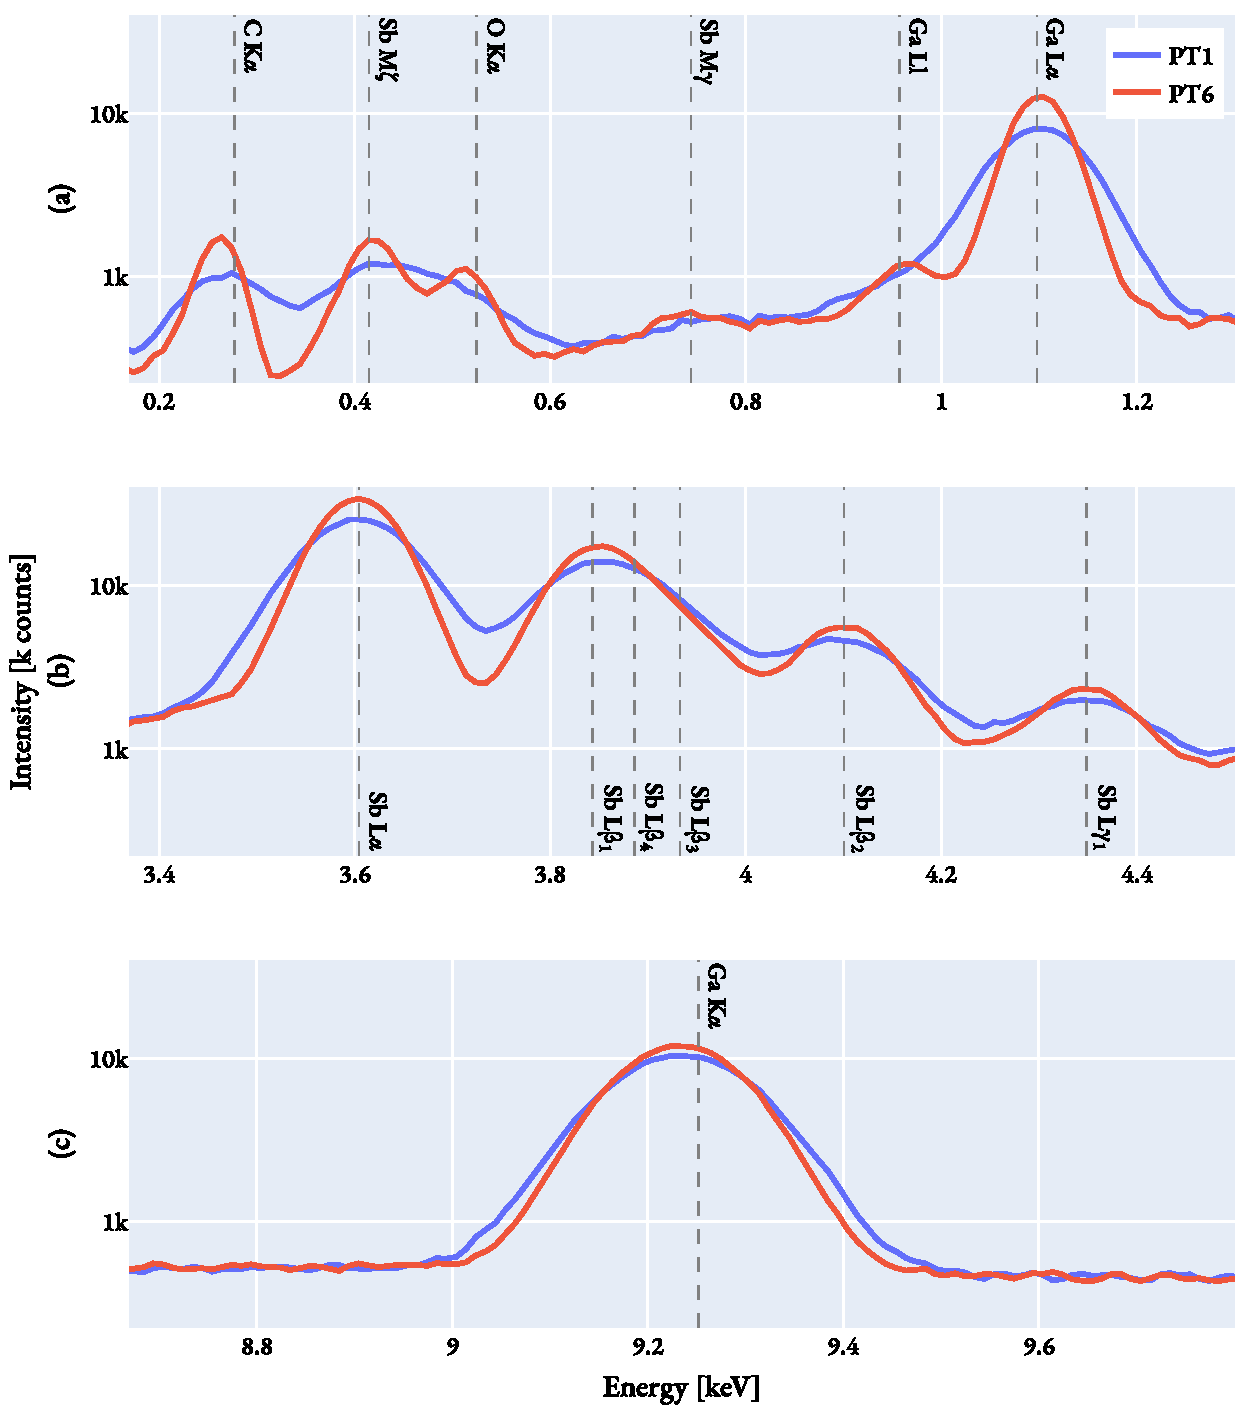
\includegraphics[width=0.95\linewidth]{figures/results/eds_energyResolutions_process_time.pdf}
    \caption{
        Different energy resolutions on the same specimen, because of different process times.
        The maximum (red) and minimum (blue) PT on the instrument is used.
        $E_0$ = 30 kV, $I_b$ = 50 pA for both spectra.
        The PT 1 and PT 4 spectra are not shown, but are in between the PT 2 and PT 6 spectra.
        Panel (a) is the spectrum at low energy, where the effect most influential.
        With PT 1 the Sb M$\eta$ and O K$\alpha$ peak are merged, and the Ga L$l$ and Ga L$\alpha$ peaks are merged.
        Panel (b) is the spectrum at medium energy, where the effect less influential, but the peak contrast is lowered.
        Panel (c) is the spectrum at high energy, where the effect is almost negligible.
        All three panels span 1.13 keV and have the same range of counts.
        The vertical lines are the theoretical line energies.
    }
    \label{fig:results:energy_resolutions_process_time}
\end{figure}


The effect of the process time on the FWHM of the lines is shown in \cref{tab:results:PTvsFWHMs}.
The table shows the measured FWHM of Ga L$\alpha$, Sb L$\alpha$, and Ga K$\alpha$ for different process times.
The measurement is done on the Gaussian fit of the peaks.
Additionally, the FWHM of the Mn K$\alpha$ is estimated for each process time.
The table shows the variations on the GaSb specimen with PT 1, 2, 4, and 6.
The last row shows the FWHM in the GaAs specimen at PT 6 for reference.
All spectra in the table were acquired at 30 kV and 50 pA.
In the GaSb spectra, the PT 1 has DT 4\%, PT 2 has DT 7\%, PT 4 has DT 13\%, and PT 6 has DT 44\%.
The GaAs spectrum with PT 6 has DT 44\%.

% TODO discuss: based on the numbers, PT 4 should be good enough for most applications. High resolution, and much faster than PT 6. DT44 is really high, and not nice for mapping.
% TODO discuss: specimen with many L-lines


\begin{table}[phtb]
    \begin{center}
        \caption{
            FWHMs of lines with different process times.
            All the FWHMs are in eV, calculated from the Gaussian fit.
            All spectra are acquired at 30 kV and 50 pA.
            GaSb is used as the specimen, except for the last column, where GaAs is used for reference.
        }
        \renewcommand*{\arraystretch}{1.4}
        \label{tab:results:PTvsFWHMs}
        \begin{tabular}{rrrrrr}
            \hline
            \textbf{Line}       & \textbf{PT 1} & \textbf{PT 2} & \textbf{PT 4} & \textbf{PT 6} & \textbf{PT 6, GaAs} \\
            \hline
            %C K$\alpha$&&&&&\\ % C is not it the models used
            Ga L$\alpha$        & 109           & 88            & 73            & 65            & 67                  \\
            Sb L$\alpha$        & 138           & 122           & 108           & 102           & -                   \\
            Mn K$\alpha$ (est.) & 158           & 143           & 132           & 127           & 129                 \\
            Ga K$\alpha$        & 182           & 172           & 165           & 161           & 163                 \\
            \hline
        \end{tabular}
    \end{center}
\end{table}



\subsection{Beam energy and beam current}
\label{results:beam_energy_and_beam_current}


% comment on (A) and (B)
The energy and the amount of electrons in the probe is important for the emerging X-ray spectrum.
Using a low overvoltage is both problematic for the qualitative and quantitative analysis.
The green line in \cref{fig:results:GaAs_voltages} is the 10 kV spectrum for GaAs, which has no visible signal from the Ga K$\alpha$ peak, where the overvoltage is around 1.1.
The overvoltage is also an issue for the Sb L-lines in the 5 kV spectrum in \cref{fig:results:GaSb_voltages}.
The Sb L-peaks are present, but weak, and the L$l$ peak is not visible.
This issue with the weak Sb-L peaks makes the quantification of Sb difficult at low voltages, as seen further down in \cref{results:initial_quantification}.
The GaAs specimen is quantified much more accurately at 5 kV, because the Ga L$\alpha$ and As L$\alpha$ peaks have similar overvoltages.
In the voltage series, which are group (A) and (B) in \cref{method:acquisition_settings}, the amount of counts in the lower voltages are quite low.
The low amount of counts is due to keeping the beam current constant at 50 and 25 pA.
Using a higher beam current on the lower energies would have made normalization more necessary, which is adding a layer of subjective decisions as the spectra must be normalized to something.
% TODO discuss: this might not have been the best choice. For future work one can try to get the same ICR for all voltages, and see if the results are better and still comparable, without normalization.
Even though the 30 kV spectra in GaAs and GaSb have more counts and are smoother than the other spectra, they both have more artifacts.
% TODO discuss: the amount of artifacts have to be adjusted for the specimen and the goal of the analysis.
Around 1 keV, the 30 kV and 15 kV spectra are quite similar.
% TODO discuss: at 1 keV, the ionization cross section when using 15 or 30 kV is more or less the same.

\brynjar{TODO: write something about ICR?}

% (C) (D) and (E)
As the 30 and 15 kV spectra gave better results for GaSb, they were chosen for group (C), (D), and (E).
In (C) different process times were tested, and these results are presented in \cref{results:process_time}.
In (D) different beam currents were tested, while also changing the PT and $E_0$.
In (E) the data type maps were acquired.
% (D)
The combination of high $i_b$ and high PT in two of the spectra in (D) made the DT very high.
Despite the high DT, the amount of artifacts in the 200 pA and 400 pA spectra were similar to the 50 pA spectra.
However, with DT at 53\% and 77\%, the acquisition time was very long.
% TODO discuss: DT is not a good measure of the artifacts, at least not when using high PT which allows the electronics to count accurately. However, high i_b and PT is bad for mapping.
On the quantification presented in \cref{results:initial_quantification}, the beam energy appears to be more important than the beam current.
% TODO discuss: this might be a result of the lines used (Ga L or Ga K).
\brynjar{TODO: the maps have not been analyzed properly yet.}








\subsection{Duane-Hunt limit}
\label{results:duane_hunt}

The Duane-Hunt limits, or the effective beam energies, are presented in \cref{tab:results:duane_hunt}.
The table shows the Duane-Hunt limit for the 5, 10, and 15 kV spectra.
As the energy range recorded in the spectra were 0-20 keV, the Duane-Hunt limit of the 30 kV spectra were not possible to calculate.
All the calculated Duane-Hunt limits are within 0.2 keV of the nominal beam energy, i.e. the specified beam energy in the SEM software.
The average deviation is 0.06 keV, with a standard deviation of 0.04 keV.
This shows that the beam energy is quite stable.
% TODO discuss: the usefulness of calculating the DH limit.

\begin{table}[htbp]
    \begin{center}
        \caption{
            The Duane-Hunt limit in the sub 30 kV spectra.
            All spectra are acquired with PT 6.
        }
        % \renewcommand*{\arraystretch}{1.4}
        \label{tab:results:duane_hunt}
        \begin{tabular}{rrrrr}
            \hline
            \textbf{Group} & \textbf{Specimen} & \textbf{$E_0$} & \textbf{$i_b$} & \textbf{Duane-Hunt limit} \\
            \emph{}        & \emph{}           & \emph{[kV]}    & \emph{[pA]}    & \emph{[kV]}               \\
            \hline
            A              & GaAs              & 5              & 25             & 4.92                      \\
            A              & GaAs              & 10             & 25             & 10.08                     \\
            A              & GaAs              & 15             & 25             & 14.98                     \\
            B              & GaSb              & 5              & 50             & 4.86                      \\
            B              & GaSb              & 10             & 50             & 10.05                     \\
            B              & GaSb              & 15             & 50             & 14.99                     \\
            D              & GaSb              & 15             & 200            & 15.03                     \\
            D              & GaSb              & 15             & 400            & 15.1                      \\
            \hline
        \end{tabular}
    \end{center}
\end{table}
}




\subsection{Fiori P/B ratio}
\label{results:fiori}

The Fiori numbers are presented in \cref{tab:results:fiori}, with the Fiori P/B ratio in the five rightmost columns.
% # for Ga La, Ga Ka, As La, Sb La, Sb Lb
The ratios are for the Ga L$\alpha$, Ga K$\alpha$, As L$\alpha$, Sb L$\alpha$, and Sb L$\beta$.
The Fiori P/B ratios have a spread between just below 100 to right under 800.
The overall highest ratio is for the Ga K$\alpha$ peak for the 30 kV and 25 pA GaAs spectrum, with a ratio of 770.
% TODO discuss: repeat why the numbers are so high. That is dividing by one single bg channel, which makes the ratio unaffected by energy resolution.
The equal settings in the GaSb spectrum have a ratio of 408 for the Ga K$\alpha$ peak.
For the Ga K$\alpha$ peaks, the GaAs spectrum have almost twice as high Fiori P/B ratios as the GaSb spectrum.
The Ga L$\alpha$ peak is present in all the spectra, and it can be used for comparison.
However, the background counts around the Ga L$\alpha$ peak is around 2-5 times higher in the GaSb spectra than in the GaAs spectra, which is reflected in the different Fiori ratios for the Ga L$\alpha$ peak.
% TODO discuss: the mu_rho of GaAs is much higher than GaSb above 1 keV because of the double absorption edge. This gives a much higher Fiori ratio for GaAs than GaSb, as the background is lower. But the Ga_La peak ing GaAs is also higher. The specimen dependness is high.
The peak height between GaAs and GaSb differs some, but it is probably the background levels which make the biggest impact on the Fiori P/B ratios.
For the Ga L$\alpha$ peak, the Fiori P/B ratios is up to 6 times higher for GaAs than GaSb.
This shows clearly that the Fiori P/B ratio is specimen dependent, even when using the same peak and setting.


% what affects the Fiori numbers
The data acquired gives indications of what affects the Fiori numbers.
The two 30 kV GaAs spectra at 25 pA and 50 pA have the highest Fiori numbers.
Even though the 50 pA spectrum has more than twice the amount of maximum counts in the Ga L$\alpha$ peak compared to the 25 pA spectrum, their Fiori numbers are quite similar.
Both these 30 kV spectra have PT 6, but the 50 pA spectrum has a higher DT at 44\%, while the 25 pA spectrum has a DT of 25\%.
% TODO discuss: the very similar Fiori numbers imply that the spectra are equally good. Put this into context with the quantification results and the DT, as this increase acquisition time. Implies that there is a threshold where more counts does not give better results, and maybe the Fiori ratio is a good measure of this.
% TODO discuss: high Fiori does not mean good quantification. GaSb are closer to 50\% by AZtec (and me?), but the GaAs Fiori numbers are in general higher.
The different PTs tested on GaSb in (C) and (D) does not seem to have a noticeable effect with a trend in either direction.
An increase in $i_b$ appears to have a decreasing effect on the Fiori numbers, but the effect is small.
This $i_b$ effect can be seen on the three 15 kV GaSb spectra, with 50 pA, 200 pA, and 400 pA.
The same effect is visible for the 30 kV GaSb spectra taken with 50 pA and 400 pA at PT 1, with the Ga L$\alpha$ peak as an exception.
However, the biggest effect and trend appears to come from $E_0$.
For the GaAs specimen, the Fiori P/B ratio of Ga L$\alpha$ increase with increasing $E_0$.
The same $E_0$ effect is visible for the Ga K$\alpha$, Sb L$\alpha$, and Sb L$\beta$ peaks in the GaSb spectra.
The Ga L$\alpha$ peak in the GaSb spectra does not follow this trend, but this ratio is changing much less than the ratios for the three other peaks.
% TODO discuss: the Fiori P/B is a function of the specimen (maybe most important?), the beam energy (much), the beam current (not much). Additionally, the calculation method is very important. And the detector is also a factor, but different detectors have not been tested in this work.


% TODO discuss: what range of values is good for the Fiori number? And say something about GaAs having higher number, but being quantified less accurately.


\begin{table}[hbtp]
    \begin{center}
        \caption{
            The Fiori P/B ratios.
            Group A is GaAs, which is sorted by the Ga L$\alpha$ ratio.
            Group B, C, and D is GaSb, which is sorted by the Sb L$\alpha$ ratio.
            The "-" indicates that the line is not present in the spectrum.
        }
        %\renewcommand*{\arraystretch}{1.4}
        \label{tab:results:fiori}
        \begin{tabular}{rrrrrrrrr}
            \hline
            \textbf{Group} & \textbf{$E_0$} & \textbf{$i_b$} & \textbf{PT} & \textbf{Fiori P/B}    & \textbf{Fiori P/B}    & \textbf{Fiori P/B}    & \textbf{Fiori P/B}    & \textbf{Fiori P/B}   \\
            \emph{}        & \emph{[kV]}    & \emph{[pA]}    & \emph{}     & \textbf{Ga L$\alpha$} & \textbf{Ga K$\alpha$} & \textbf{As L$\alpha$} & \textbf{Sb L$\alpha$} & \textbf{Sb L$\beta$} \\
            \hline
            A              & 30             & 50             & 6           & 586                   & 762                   & 236                   & -                     & -                    \\
            A              & 30             & 25             & 6           & 573                   & 770                   & 233                   & -                     & -                    \\
            A              & 15             & 25             & 6           & 414                   & 187                   & 250                   & -                     & -                    \\
            A              & 10             & 25             & 6           & 280                   & 0                     & 206                   & -                     & -                    \\
            A              & 5              & 25             & 6           & 155                   & -                     & 140                   & -                     & -                    \\
            \hline
            C              & 30             & 50             & 4           & 87                    & 407                   & -                     & 386                   & 169                  \\
            C              & 30             & 50             & 2           & 84                    & 414                   & -                     & 386                   & 169                  \\
            C              & 30             & 50             & 1           & 83                    & 414                   & -                     & 386                   & 168                  \\
            B              & 30             & 50             & 6           & 86                    & 408                   & -                     & 385                   & 168                  \\
            D              & 30             & 400            & 1           & 86                    & 320                   & -                     & 360                   & 156                  \\
            B              & 15             & 50             & 6           & 110                   & 138                   & -                     & 215                   & 97                   \\
            D              & 15             & 200            & 6           & 109                   & 131                   & -                     & 214                   & 97                   \\
            D              & 15             & 400            & 6           & 107                   & 124                   & -                     & 211                   & 95                   \\
            B              & 10             & 50             & 6           & 113                   & 9                     & -                     & 140                   & 65                   \\
            B              & 5              & 50             & 6           & 91                    & -                     & -                     & 16                    & 5                    \\
            \hline
        \end{tabular}
    \end{center}
\end{table}
}



\subsection{Portion of counts in the peaks}
\label{results:portion_of_counts}

\brynjar{Something about the portion of counts in the peaks vs. in the background.}

\clearpage

















% 4.4
\section{Quantitative analysis}
\label{results:quantitative}


\brynjar{Intro?}


\subsection{Initial quantification}
\label{results:initial_quantification}

% initial quantification (AZtec and i/i_sum)
Initial quantification was done with the AZtec software and with the uncorrected area ratio method.
The area ratio method gives relative compositions, and it is described in \cref{theory:quantitative:principle}, with \cref{eq:theory:quantitative:area_ratio}.
AZtec too gives relative compositions, based on the elements confirmed to be present in the spectrum.
The initial quantification results are shown in \cref{tab:results:initial_quantification}, and plotted in \cref{fig:results:initial_quantification}.
Statistical numbers for the results are shown in \cref{tab:results:stats_initial_quantification}.
\ton{I decided to round the percentages to integers. OK?}
As the table and figure show, some results are close to 50\%.
In 13 of the 15 spectra, AZtec gives a result at 50$\pm2$\%, and 2 of the results are at 50$\pm4$\%.
The 5 area ratios from GaSb spectra with $E_0$ = 30 kV are at 50$\pm2$\%.
The three 15 kV results from GaSb have a deviation of $\pm$ 10\%, which show the need for some correction.
The remaining results from the area ratio method produce results with higher deviations, strongly implying the need for corrections.
% The low energy results from GaAs have a high deviation, probably due to issues with overvoltage.

% TODO discuss: AZtec is pretty good, but misses at eg 5kV GaSb
% TODO discuss: the uncorrected results are good for some spectra, but others are bad. Overvoltage might be the main reason.
% TODO discuss: also comparing Ga Ka with Sb La, which should have different omega (ref to image in theory)
% TODO discuss: bulk corrections is needed

\newgeometry{top=2cm} % change the margins to fit the table.

\begin{table}[phtb]
    \begin{center}
        \caption{
            Initial quantification in selected spectra.
            Compositions from AZtec and the intensity ratio method.
            Each spectrum corresponds to two lines, one for each element.
            The table is summarized in \cref{tab:results:initial_quantification_stats}.
        }
        %\renewcommand*{\arraystretch}{1.4}
        \label{tab:results:initial_quantification}
        \begin{tabular}{rrrrrrrr}
            \hline
            \textbf{ Group} & \textbf{Line} & \textbf{$E_0$} & \textbf{$i_b$} & \textbf{PT} & \textbf{Intensity} & \textbf{AZtec comp.} & \textbf{Intensity ratio comp.} \\
            \emph{}         & \emph{}       & \emph{[kV]}    & \emph{[pA]}    & \emph{}     & \emph{[k counts]}  & \emph{at\%}          & \emph{at\%}                    \\
            \hline
            A               & As L$\alpha$  & 5              & 25             & 6           & 13                 & 53                   & 43                             \\
            A               & Ga L$\alpha$  & 5              & 25             & 6           & 16                 & 47                   & 57                             \\
            A               & As L$\alpha$  & 10             & 25             & 6           & 37                 & 52                   & 40                             \\
            A               & Ga L$\alpha$  & 10             & 25             & 6           & 51                 & 48                   & 60                             \\
            A               & As L$\alpha$  & 15             & 25             & 6           & 62                 & 51                   & 36                             \\
            A               & Ga L$\alpha$  & 15             & 25             & 6           & 103                & 49                   & 64                             \\
            A               & As K$\alpha$  & 30             & 25             & 6           & 84                 & 48                   & 36                             \\
            A               & Ga K$\alpha$  & 30             & 25             & 6           & 141                & 52                   & 64                             \\
            A               & As K$\alpha$  & 30             & 50             & 6           & 180                & 48                   & 36                             \\
            A               & Ga K$\alpha$  & 30             & 50             & 6           & 303                & 52                   & 64                             \\
            \hline
            B               & Ga L$\alpha$  & 5              & 50             & 6           & 19                 & 39                   & 97                             \\
            B               & Sb L$\alpha$  & 5              & 50             & 6           & 1                  & 61                   & 3                              \\
            B               & Ga L$\alpha$  & 10             & 50             & 6           & 46                 & 47                   & 75                             \\
            B               & Sb L$\alpha$  & 10             & 50             & 6           & 27                 & 53                   & 25                             \\
            B               & Ga L$\alpha$  & 15             & 50             & 6           & 74                 & 49                   & 58                             \\
            B               & Sb L$\alpha$  & 15             & 50             & 6           & 94                 & 51                   & 42                             \\
            B               & Ga K$\alpha$  & 30             & 50             & 6           & 191                & 50                   & 48                             \\
            B               & Sb L$\alpha$  & 30             & 50             & 6           & 359                & 50                   & 52                             \\
            \hline
            C               & Ga K$\alpha$  & 30             & 50             & 4           & 189                & 50                   & 48                             \\
            C               & Sb L$\alpha$  & 30             & 50             & 4           & 350                & 50                   & 52                             \\
            C               & Ga K$\alpha$  & 30             & 50             & 2           & 184                & 50                   & 49                             \\
            C               & Sb L$\alpha$  & 30             & 50             & 2           & 330                & 50                   & 51                             \\
            C               & Ga K$\alpha$  & 30             & 50             & 1           & 178                & 50                   & 51                             \\
            C               & Sb L$\alpha$  & 30             & 50             & 1           & 304                & 50                   & 49                             \\
            \hline
            D               & Ga L$\alpha$  & 15             & 200            & 6           & 155                & 49                   & 57                             \\
            D               & Sb L$\alpha$  & 15             & 200            & 6           & 200                & 51                   & 43                             \\
            D               & Ga L$\alpha$  & 15             & 400            & 6           & 284                & 49                   & 57                             \\
            D               & Sb L$\alpha$  & 15             & 400            & 6           & 367                & 51                   & 43                             \\
            D               & Ga K$\alpha$  & 30             & 400            & 1           & 1724               & 50                   & 50                             \\
            D               & Sb L$\alpha$  & 30             & 400            & 1           & 2996               & 50                   & 50                             \\
            %
            %E&Map&&&&&&\\
            %E&Map&&&&&&\\
            %&&&&&&&\\
            \hline
        \end{tabular}
    \end{center}
\end{table}
\restoregeometry % put the margins back to normal
\begin{table}[phtb]
    \begin{center}
        \caption{
            Numbers for the at\% deviations in the initial quantification, see \cref{tab:results:initial_quantification}
            The GaSb 5 kV spectrum is excluded from the numbers, as it is viewed as an outlier.
            The table gives the average deviation in at\% from 50 at\%, for GaAs and GaSb seperated.
            The number of deviations below 5 at\% and above 10 at\% are also tabulated.
        }
        %\renewcommand*{\arraystretch}{1.4}
        \label{tab:results:initial_quantification_stats}
        \begin{tabular}{rrrr}
            \hline
            \textbf{Specimen} & \textbf{Number}         & \textbf{AZtec} & \textbf{Intensity ratio} \\
            \hline
            GaAs              & Average deviation, at\% & 2 at\%         & 12 at\%                  \\
                              & Deviations $>10$ at\%   & 0              & 4                        \\
                              & Deviations  $<5$  at\%  & 5              & 0                        \\
            \hline
            GaSb              & Average deviation, at\% & 1 at\%         & 6 at\%                   \\
                              & Deviations $>10$ at\%   & 0              & 1                        \\
                              & Deviations  $<5$  at\%  & 9              & 5                        \\

            \hline
        \end{tabular}
    \end{center}
\end{table}



% figures/results/initial_quantification.pdf
\begin{figure}[htbp]
    \centering
    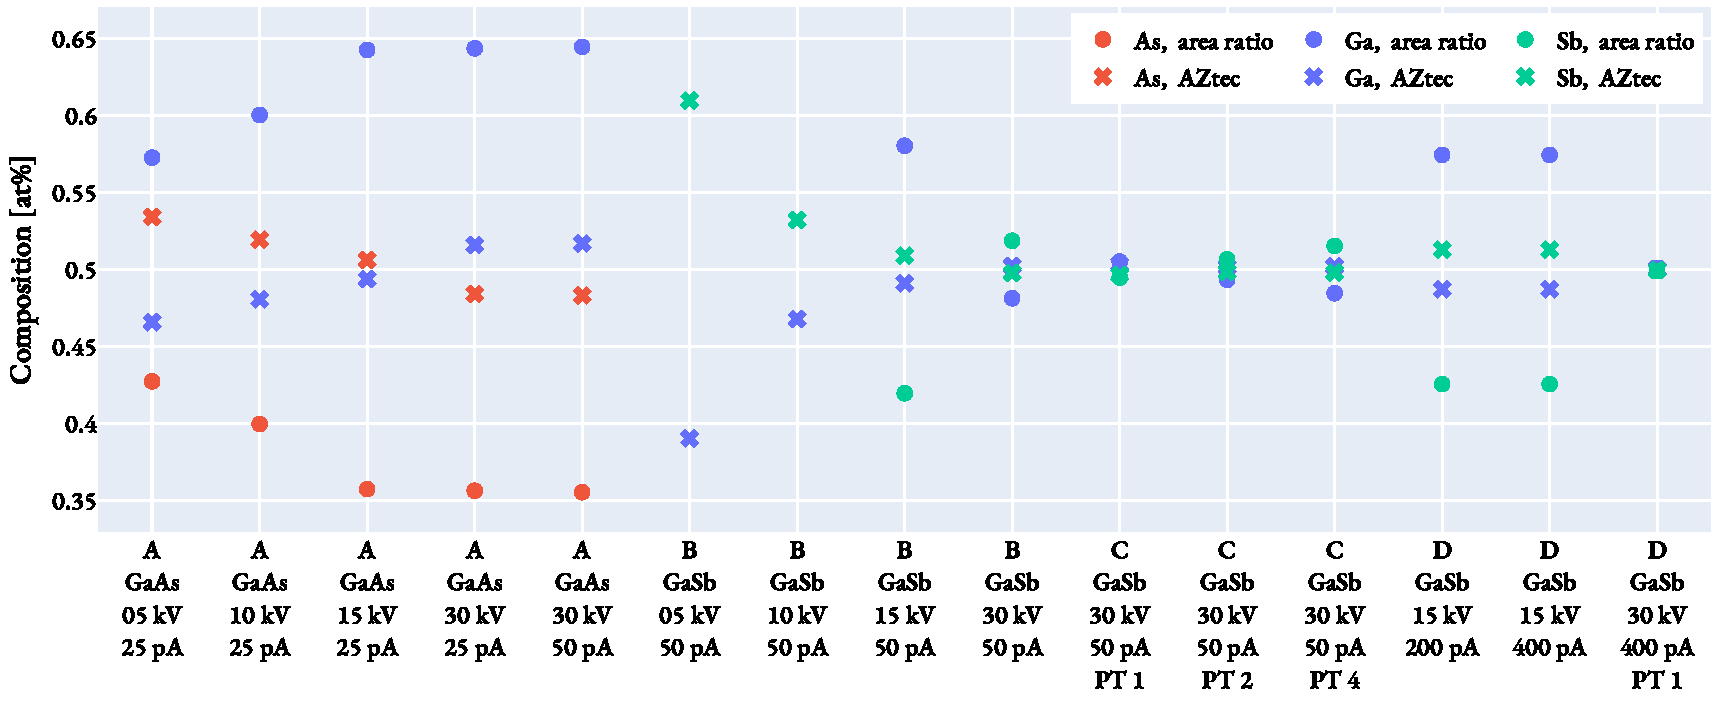
\includegraphics[width=0.99\linewidth]{figures/results/initial_quantification.pdf}
    \caption{
        Initial quantification results in at\%.
        The X markers are the quantification from AZtec.
        The circle markers are the quantification from the area ratio, without corrections.
        The group, specimen, $E_0$, $i_b$, and PT are shown on the x-axis.
        The spectra without noted PT are taken with PT 6.
        The same data is tabulated in \cref{tab:results:initial_quantification}.
    }
    \label{fig:results:initial_quantification}
\end{figure}

\ton{Are the next three paragraphs too much discussion? I would say no, but I am not sure.}

% comment on the severely poor results from GaAs at 5 kV
The GaSb spectrum at 5 kV is poorly quantified, both by AZtec and by the area ratio.
Both methods use the Ga L$\alpha$ and Sb L$\alpha$ peaks, and the Sb L$\alpha$ peak is at 3.6 keV, which is quite close to $E_0$.
The overvoltage on Sb L$\alpha$ in the 5 kV spectrum is below 1.4, while the overvoltage on the Ga L$\alpha$ is above 4.5, which results in a severely underestimated Sb content with the area ratio.
As seen in the table, the area of the Ga L$\alpha$ peak is 19 times larger than the area of the Sb L$\alpha$ peak, thus the area ratio method gives a 97:3 composition.
AZtec is doing some corrections for this, but overestimates the weight for Sb, and ends on a 39:61 composition.
The overvoltage on Sb L$\alpha$ in the 5 kV spectrum is below 1.4, while the overvoltage on the Ga L$\alpha$ is above 4.5, which results in a severely underestimated Sb content with the area ratio.
% TODO discussion: quantification on low kV of Sb and similar elements with L-peaks between 3 and 4 keV is hard. Have to do something very clever, but what?


% What corrections are needed for the area ratio?
\cref{tab:results:initial_quantification} and \cref{fig:results:initial_quantification} show that the need for corrections are varying with both specimen and acquisition parameters.
% GaAs
Different $i_b$ are not affecting the correction needs much, but the $E_0$ is.
All the GaAs spectra need corrections which increase the weight of As.
AZtec have applied corrections to the GaAs spectra, where the results are pushing As too high at 5 kV and 10 kV, and not high enough at 30 kV.
The 15 kV GaAs corrections done by AZtec on GaAs is good, resulting at 50.6:49.4.
% TODO discuss: the need to increase the weight of As is due to absoprtion of As X-rays is Ga.
% GaSb
The corrections needed in the GaSb spectra are not as clear as for GaAs.
The 30 kV GaSb spectra appears to require little corrections, and have good results with the area ratio.
The 15 kV and 10 kV spectra of GaSb need corrections to increase the weight of Sb.
The GaSb 15 kV and 10 kV spectra are quantified with Ga L$\alpha$ and Sb L$\alpha$.
% The intensity in the Sb L$\alpha$ peak in the 15 kV and 10 kV spectrum are too low, compared to the Ga L$\alpha$ peak.
AZtec have corrected the 15 kV compositions well, and semi-well for the 10 kV composition.
% TODO discuss: the need to increase the weight of Sb. The absorption should be stronger of Ga La, so this is not the reason. Probably a Z effect. Also overvoltage. Maybe omega.
Correction factors are presented in \cref{results:matrix_corrections}.

\brynjar{Move to discussion:"Since the absorption should be stronger of the Ga L$\alpha$ peak than the Sb L$\alpha$ peak, the absorption should not be the reason for the low Sb content.
    The low Sb content in the 15 kV and 10 kV spectra can be due to the overvoltage differences.
    Ga L$\alpha$ has overvoltage $U = 15/1.1 = 13.6$, and Sb L$\alpha$ has $U = 15/3.6 = 4.2$ at 15 kV.
    From the estimated ionization cross-section as a function of overvoltage, seen in \cref{fig:PAP:ionization_cross_section}, the maximum $Q(U)$ is at $U = 3.4$.
    Thus, the overvoltage at 15 kV should not be the reason for the low Sb content.
    % TODO discuss: the reason for the low Sb content at 15 kV is not the overvoltage, but something else.
    The different intensities are thus probably an effect of different Z. This should be treated somewhat by the PAP method."}






% \subsection{Quantification of SEM EDS data based on the Cliff-Lorimer method} % Tons suggested title
\subsection{Quantification of SEM EDS data as if it was TEM EDS data}
\label{sec:results:quantification_cliff_lorimer}


Quantitative analysis of the SEM EDS bulk spectra was also done under the presumption that the specimen was a TEM specimen, i.e. under the thin film approximation.
The thin film approximation assumes no absorption of the created X-rays in the specimen, and is a part of the Cliff-Lorimer (CL) method covered in \cref{sec:theory:quantitative:k_factor_vs_k_ratio}.
The presumption that the specimen is a TEM specimen was both applied in AZtec with the "TEM setting", and in HyperSpy with the CL method.
The TEM EDS quantification in AZtec is probably also done with the CL method, but it is not stated in the documentation.
TEM EDS quantification of SEM EDS data can readily be done, even though it is formally incorrect.

% the table
The results from the TEM EDS quantification routines are tabulated in \hyperref[appendix:tables]{Appendix C} in \cref{tab:results:TEM_quantification}, and statistical numbers from that table is presented in \cref{tab:results:TEM_quantification_stats}.
% TODO: check the appendix reference
% In \hyperref[appendix:tables]{Appendix C} (\cref{appendix:tables}), \cref{tab:appendix:mock_table}, the results are tabulated for all the spectra.
The calculated k-factors, which are extracted from AZtec and needed for the CL method in HyperSpy, are included in \cref{tab:results:TEM_quantification}.
The CL method in HyperSpy was done with and without the TEM absorption corrections, which is a part of the implemented CL quantification function.
The "CL*" column is without absorption corrections, and the "CL" column is with the TEM absorption corrections, where the $t$ is the set specimen thickness.
Six $t$ values were used: 50 nm, 100 nm, 200 nm, 400 nm, 1000 nm, and 10000 nm.


% comment on the severely poor results from GaAs at 5 kV
The GaSb spectrum at 5 kV is poorly quantified by AZtec.
AZtec is quantifying the 5 kV GaSb spectrum with the Ga L$\alpha$ and Sb M$\eta$ peaks.
Sb M$\eta$ is around 0.4 keV, and at such low energy the absorption is high.
AZtec does not correct for this absorption (enough at least) in TEM mode, and the resulting composition is 91:9.
The Sb M$\eta$ peak is not available in HyperSpy, and no k-factor is given for the Sb L$\alpha$ line at 5 kV.
Thus, it is not possible to quantify the 5 kV GaSb spectrum with HyperSpy.
% When using TEM mode, AZtec selects the Sb M$\eta$ line at 5 kV, and as this line is not included in HyperSpy, the 5 kV GaSb spectra were not quantified in HyperSpy.
% TODO discuss: not possible to quantify with HyperSpy at 5 kV, as the Sb M$\eta$ line is missing and thus there are no k-factor for Sb La.
% TODO discuss: HyperSpy will not give k-factors, even though some people ask for it (Gitter). This is becaues that would give a high uncertainty, as the k-factors are partly dependent on the detector.
% TODO discuss from Ton: "In discussion can debate of other more correct k-factors would lead to substantial better quantification or that own k-factors can be extracted from the data you have and if that helps, even seen the wrong preassumption"


% comment on the table values
The TEM EDS quantification results of the SEM EDS data are in general deviating from the reference value of 50:50.
The statistical numbers for \cref{tab:results:TEM_quantification} in \cref{tab:results:TEM_quantification_stats} are calculated without the 5 kV GaSb spectra, as the 5 kV spectra were not quantified in HyperSpy.
The "TEM setting" AZtec results are deviating much more from 50:50 compared to the AZtec results using the "SEM setting", presented in \cref{results:initial_quantification}.
% TODO discuss: this celarly show that AZtec is doing different quant with SEM and TEM, but the difference is not in the documentation. We know they do XPP from the blog post, and that could have been stated in the manual.
AZtec have bigger average deviations from the reference value than HyperSpy, for all quantification methods, except when $t$ = 10000 nm. 
The average AZtec deviation is 10$\pm$6\% from the reference value, where the uncertainty is the standard deviation of the deviations from 50:50.
The CL deviations start below AZtec at the uncorrected quantification, and then the average decreases as $t$ go from 50 nm to 200 nm, and then the average deviations increase again.
The three best CL quantifications are with $t$ = 100 nm (7$\pm$2 \%), $t$ = 200 nm (5$\pm$3 \%), and $t$ = 400 nm (6$\pm$4 \%).
The number of deviations above 10\% and below 5\% are also presented in \cref{tab:results:TEM_quantification_stats}, where 14 is the total number of spectra.
CL with $t$ = 100 nm have zero deviations above 10\%, but only one below 5\%.
CL with $t$ = 200 nm have one deviation above 10\%, and five below 5\%.
CL with $t$ = 400 nm have one deviation above 10\%, and four below 5\%.
% TODO discuss: the numbers above 10 and below 5 is nice, because the average is not the whole story. I would say t = 200 nm is the best, because it has a low average deviation, and good numbers for >10 and <5. The 200 nm also perform most similar on the GaAs and GaSb, which is important.
% TODO discuss: HyperSpy is actually better than AZtec, on TEM setting. Also, it is a special case, other specimen might have very different results.

\ton{Now the statistical number table is placed here, and the result table in the appendix. Is that good? The result table is so huge that it is not easy to read.}

\begin{table}[phtb]
    \begin{center}
        \caption{
            Numbers for the at\% deviations with the thin film assumption, i.e. the TEM quantification routines.
            The table is a summary of \cref{tab:results:TEM_quantification}.
            The AZtec result is from the "TEM EDS setting", and the CL results are from the Cliff-Lorimer method in HyperSpy.
            CL* is without corrections, the others CL have absorption correction with input thicknesses $t$, in nm.
        }
        %\renewcommand*{\arraystretch}{1.4}
        \label{tab:results:TEM_quantification_stats}
        \begin{tabular}{rrrrrrrrrr}
            \hline
            \textbf{Specimen} & \textbf{Number}         & \textbf{AZtec} & \textbf{CL*} & \textbf{CL}   & \textbf{CL}    & \textbf{CL}    & \textbf{CL}    & \textbf{CL}   & \textbf{CL}    \\
            \emph{}           & \emph{}                 & \emph{TEM}        & \emph{}      & \emph{$t$=50} & \emph{$t$=100} & \emph{$t$=200} & \emph{$t$=400} & \emph{$t$=1k} & \emph{$t$=10k} \\
            \hline
            GaAs              & Average deviation, at\% & 8 at\%         & 9 at\%       & 8 at\%        & 7 at\%         & 5 at\%         & 5 at\%         & 7 at\%        & 6 at\%         \\
                              & Deviations $>10$ at\%   & 1              & 1            & 1             & 0              & 0              & 0              & 0             & 2              \\
                              & Deviations  $<5$  at\%  & 1              & 1            & 1             & 1              & 2              & 3              & 1             & 2              \\
            \hline
            GaSb              & Average deviation, at\% & 11 at\%        & 9 at\%       & 8 at\%        & 7 at\%         & 5 at\%         & 7 at\%         & 11 at\%       & 21 at\%        \\
                              & Deviations $>10$ at\%   & 3              & 3            & 0             & 0              & 1              & 1              & 4             & 9              \\
                              & Deviations  $<5$  at\%  & 0              & 1            & 0             & 0              & 3              & 1              & 5             & 0              \\
            \hline
        \end{tabular}
    \end{center}
\end{table}















\subsection{Matrix corrections}
\label{results:matrix_corrections}



\subsubsection{ZAF absorption corrections}
\label{results:matrix_corrections:ZAF}

The ZAF absorption corrections were done with \cref{eq:theory:quantitative:absorption}. %, and the results are presented in \cref{tab:results:ZAF_corrections_factors} and \cref{tab:results:ZAF_corrections_compositions}.
The calculated maximum electron range $r$ is presented in \cref{tab:results:ZAF_corrections_range_r}.
% The parameters are line, elements, $\mu_\rho$, $\rho$, $E_0$, assumed atomic fraction, TOA, and maximum electron range $t$.
To calculate the absorption correction factors, $r$ is divided by 2, 3, and 4 to get different approximations for the average depth of origin of the X-rays.
The calculated absorption correction factors are presented in \cref{tab:results:ZAF_corrections_factors}.
The corrected compositions are presented in \cref{tab:results:ZAF_corrections_compositions}.
Statistical numbers for the compositions are given in \cref{tab:results:ZAF_corrections_compositions_stats}.

\ton{Should I drop the GaSb absorption corrections? They only make the results worse.}

\ton{Should I also have average etc. here? For GaSb the results are bad (does not need the absorption correction), but for GaAs the results are improved.}

\ton{TODO: the densities are not the same as stated on Wikipedia.}


\begin{table}[htbp]
    \begin{center}
        \caption{
            Selected maximum ranges of creation for lines in different specimen, based on the Kanaya-Okayama parameterization.
            The path length of the X-rays are $r \cdot \csc(TOA)$.
            The ranges are used to calculate the ZAF absorption correction factors, listed in \cref{tab:results:ZAF_corrections_factors}.
        }
        %\renewcommand*{\arraystretch}{1.4}
        \label{tab:results:ZAF_corrections_range_r}
        \begin{tabular}{rrrrrr}
            \hline
            \textbf{Specimen} & \textbf{Line} & \textbf{$r$ at 30 kV} & \textbf{$r$ at 15 kV} & \textbf{$r$ at 10 kV} & \textbf{$r$ at 5 kV} \\
            \emph{}           & \emph{}       & \emph{[\textmu m]}    & \emph{[\textmu m]}    & \emph{[\textmu m]}    & \emph{[\textmu m]}   \\
            \hline
            GaAs              & Ga L$\alpha$  & 4.13                  & 1.29                  & 0.65                  & 0.19                 \\
                              & As L$\alpha$  & 4.12                  & 1.28                  & 0.64                  & 0.19                 \\
                              & Ga K$\alpha$  & 3.56                  & 0.72                  & 0.08                  & -                    \\
            %&As K$\alpha$&&&&\\
            \hline
            GaSb              & Ga L$\alpha$  & 4.02                  & 1.25                  & 0.63                  & 0.19                 \\
                              & Sb L$\alpha$  & 3.92                  & 1.15                  & 0.53                  & 0.09                 \\
            %&Ga K$\alpha$&&&&\\
            \hline
        \end{tabular}
    \end{center}
\end{table}

\begin{table}[phtb]
    \begin{center}
        \caption{
            Absorption correction factors from the ZAF method used.
            The absorption correction factors are in the three rightmost colums, idicated by "A t/x", where x is the number that the maximum electron range is divided by.
            Similar specimen, line, and $E_0$ have the same A, thus some of the duplicated spectra are removed.
        }
        %\renewcommand*{\arraystretch}{1.4}
        \label{tab:results:ZAF_corrections_factors}
        \begin{tabular}{rrrrrr}
            \hline
            \textbf{ Group} & \textbf{Line} & \textbf{$E_0$} & \textbf{A with t/2} & \textbf{A with t/3} & \textbf{A t/4} \\
            \emph{}         & \emph{}       & \emph{[kV]}    & \emph{}        & \emph{}        & \emph{}        \\
            \hline
            A               & As L$\alpha$  & 5              & 1.54           & 1.33           & 1.24           \\
            A               & Ga L$\alpha$  & 5              & 1.18           & 1.12           & 1.09           \\
            A               & As L$\alpha$  & 10             & 3.93           & 2.49           & 1.98           \\
            A               & Ga L$\alpha$  & 10             & 1.69           & 1.42           & 1.30           \\
            A               & As L$\alpha$  & 15             & 14.79          & 6.02           & 3.85           \\
            A               & Ga L$\alpha$  & 15             & 2.80           & 1.99           & 1.67           \\
            A               & As K$\alpha$  & 30             & 1.33           & 1.21           & 1.15           \\
            A               & Ga K$\alpha$  & 30             & 1.11           & 1.07           & 1.05           \\
            %A&As K$\alpha$&30&1.33&1.21&1.15\\
            %A&Ga K$\alpha$&30&1.11&1.07&1.05\\
            \hline
            B               & Ga L$\alpha$  & 5              & 1.73           & 1.44           & 1.32           \\
            B               & Sb L$\alpha$  & 5              & 1.05           & 1.03           & 1.03           \\
            B               & Ga L$\alpha$  & 10             & 5.72           & 3.20           & 2.39           \\
            B               & Sb L$\alpha$  & 10             & 1.17           & 1.11           & 1.08           \\
            B, D            & Ga L$\alpha$  & 15             & 31.00          & 9.87           & 5.57           \\
            B, D            & Sb L$\alpha$  & 15             & 1.37           & 1.23           & 1.17           \\
            B, C, D         & Ga K$\alpha$  & 30             & 1.33           & 1.21           & 1.16           \\
            B, C, D         & Sb L$\alpha$  & 30             & 2.71           & 1.94           & 1.65           \\
            % \hline          &               &                &                &                &                \\
            %C&Ga K$\alpha$&30&1.33&1.21&1.16\\
            %C&Sb L$\alpha$&30&2.71&1.94&1.65\\
            %C&Ga K$\alpha$&30&1.33&1.21&1.16\\
            %C&Sb L$\alpha$&30&2.71&1.94&1.65\\
            %C&Ga K$\alpha$&30&1.33&1.21&1.16\\
            %C&Sb L$\alpha$&30&2.71&1.94&1.65\\
            % \hline          &               &                &                &                &                \\
            %D&Ga K$\alpha$&30&1.33&1.21&1.16\\
            %D&Sb L$\alpha$&30&2.71&1.94&1.65\\
            %D&Ga L$\alpha$&15&31.00&9.87&5.57\\
            %D&Sb L$\alpha$&15&1.37&1.23&1.17\\
            %D&Ga L$\alpha$&15&31.00&9.87&5.57\\
            %D&Sb L$\alpha$&15&1.37&1.23&1.17\\
            %
            %E&Map&&&&\\
            %E&Map&&&&\\
            %&&&&&\\
            \hline
        \end{tabular}
    \end{center}
\end{table}

\newgeometry{top=2cm} % change the margins to fit the table.
\begin{table}[phtb]
    \begin{center}
        \caption{
            Compositions from the intensity ratio method with absorption corrected intensities. The uncorrected at.\% value is tabulated for reference.
            See \cref{tab:results:ZAF_corrections_factors} for the correction factors.
            Average numbers are given in \cref{tab:results:ZAF_corrections_compositions_stats}.
            Each spectrum has two lines in the table.
        }
        %\renewcommand*{\arraystretch}{1.4}
        \label{tab:results:ZAF_corrections_compositions}
        \begin{tabular}{rrrrrrrr}
            \hline
            \textbf{Groups} & \textbf{Line} & \textbf{$E_0$} & \textbf{$i_b$} & \textbf{Uncorr. at.\%} & \textbf{at.\% with r/2} & \textbf{at.\% with r/3} & \textbf{at.\% with r/4} \\
            \emph{}         & \emph{}       & \emph{[kV]}    & \emph{[pA]}    & \emph{}                & \emph{}                 & \emph{}                 & \emph{}                 \\
            \hline
            A               & As L$\alpha$  & 5              & 25             & 43                     & 48                      & 46                      & 45                      \\
            A               & Ga L$\alpha$  & 5              & 25             & 57                     & 52                      & 54                      & 55                      \\
            A               & As L$\alpha$  & 10             & 25             & 40                     & 58                      & 52                      & 49                      \\
            A               & Ga L$\alpha$  & 10             & 25             & 60                     & 42                      & 48                      & 51                      \\
            A               & As L$\alpha$  & 15             & 25             & 36                     & 71                      & 60                      & 54                      \\
            A               & Ga L$\alpha$  & 15             & 25             & 64                     & 29                      & 40                      & 46                      \\
            A               & As K$\alpha$  & 30             & 25             & 36                     & 39                      & 38                      & 37                      \\
            A               & Ga K$\alpha$  & 30             & 25             & 64                     & 61                      & 62                      & 63                      \\
            A               & As K$\alpha$  & 30             & 50             & 36                     & 39                      & 38                      & 37                      \\
            A               & Ga K$\alpha$  & 30             & 50             & 64                     & 61                      & 62                      & 63                      \\
            \hline
            B               & Ga L$\alpha$  & 5              & 50             & 97                     & 98                      & 98                      & 98                      \\
            B               & Sb L$\alpha$  & 5              & 50             & 3                      & 2                       & 2                       & 2                       \\
            B               & Ga L$\alpha$  & 10             & 50             & 75                     & 93                      & 89                      & 86                      \\
            B               & Sb L$\alpha$  & 10             & 50             & 25                     & 7                       & 11                      & 14                      \\
            B               & Ga L$\alpha$  & 15             & 50             & 58                     & 97                      & 91                      & 86                      \\
            B               & Sb L$\alpha$  & 15             & 50             & 42                     & 3                       & 9                       & 14                      \\
            B               & Ga K$\alpha$  & 30             & 50             & 48                     & 32                      & 37                      & 40                      \\
            B               & Sb L$\alpha$  & 30             & 50             & 52                     & 68                      & 63                      & 60                      \\
            \hline
            C               & Ga K$\alpha$  & 30             & 50             & 48                     & 32                      & 37                      & 40                      \\
            C               & Sb L$\alpha$  & 30             & 50             & 52                     & 68                      & 63                      & 60                      \\
            C               & Ga K$\alpha$  & 30             & 50             & 49                     & 33                      & 38                      & 41                      \\
            C               & Sb L$\alpha$  & 30             & 50             & 51                     & 67                      & 62                      & 59                      \\
            C               & Ga K$\alpha$  & 30             & 50             & 51                     & 34                      & 39                      & 42                      \\
            C               & Sb L$\alpha$  & 30             & 50             & 49                     & 66                      & 61                      & 58                      \\
            \hline
            D               & Ga L$\alpha$  & 15             & 200            & 57                     & 97                      & 91                      & 86                      \\
            D               & Sb L$\alpha$  & 15             & 200            & 43                     & 3                       & 9                       & 14                      \\
            D               & Ga L$\alpha$  & 15             & 400            & 57                     & 97                      & 91                      & 86                      \\
            D               & Sb L$\alpha$  & 15             & 400            & 43                     & 3                       & 9                       & 14                      \\
            D               & Ga K$\alpha$  & 30             & 400            & 50                     & 33                      & 39                      & 41                      \\
            D               & Sb L$\alpha$  & 30             & 400            & 50                     & 67                      & 61                      & 59                      \\
            %
            %E&Map&&&&&&\\
            %E&Map&&&&&&\\
            %&&&&&&&\\
            \hline
        \end{tabular}
    \end{center}
\end{table}
\restoregeometry % put the margins back to normal

\begin{table}[phtb]
    \begin{center}
        \caption{
            Numbers for the at\% deviations from $50:50$ in the ZAF absorption corrections, in \cref{tab:results:ZAF_corrections_compositions}.
            The table gives the average and the number of deviations below 5 at\% and above 10 at\% are counted, for GaAs and GaSb separated.
            %
        }
        %\renewcommand*{\arraystretch}{1.4}
        \label{tab:results:ZAF_corrections_compositions_stats}
        \begin{tabular}{rrrrrr}
            \hline
            \textbf{Specimen} & \textbf{Numbers}        & \textbf{Uncorr.} & \textbf{ZAF A, r/2} & \textbf{ZAF A, r/3} & \textbf{ZAF A, r/4} \\
            \hline

            %GaAs&&&&&\\
            GaAs              & Average deviation, at\% & 12 at\%          & 11 at\%             & 8 at\%              & 7 at\%              \\
                              & Deviations $>10$ at\%   & 4                & 3                   & 2                   & 2                   \\
                              & Deviations  $<5$  at\%  & 0                & 1                   & 2                   & 3                   \\
            \hline
            %GaSb&&&&&\\
            GaSb              & Average deviation, at\% & 6 at\%           & 30 at\%             & 25 at\%             & 21 at\%             \\
                              & Deviations $>10$ at\%   & 1                & 9                   & 9                   & 6                   \\
                              & Deviations  $<5$  at\%  & 5                & 0                   & 0                   & 0                   \\

            \hline
        \end{tabular}
    \end{center}
\end{table}



% TODO discuss: my model is not reality. I had a bug for the range r, and when i fixed in the GaAs quantification was actually deviating more.




\subsubsection{XPP/PAP corrections}
\label{results:matrix_corrections:XPP}

% The correction factors calculated with XPP are presented in \cref{tab:results:XPP_corrections_factors}.
% These correction factors were calculated with the XPP/PAP notebook, which is in \hyperref[appendix:xpp]{Appendix B}.


The XPP/PAP corrections were done in two ways, where the measured intensity of a peak $I_A$ is divided by the calculated generated intensity of the peak $F$ or by the calculated XPP absorption correction factor $f(\chi)$.
Both ways are presented in \cref{tab:results:XPP_compositions}, where the uncorrected compositions are included for comparison.
All compositions are in atomic percent, and are calculated with the relative peak area method.
Statistical numbers for the XPP corrections are given in \cref{tab:results:XPP_compositions_stats}.
$F$ and $f(\chi)$ are calculated with the XPP/PAP notebook, and are dependent on $E_0$, $E_C$ of the line, and the elements with their weight fraction of the elements.
The elements and their weight fractions are used to calculate the density $\rho$, the mean atomic mass $M$, the mean ionization potential $J$, the mean atomic number $\bar{Z}$, the backscattering coefficient $R$, and $\mu_\rho$ of the line at $E_0$.
The weight fractions used in the calculations are set to the equivalent of a 50:50 atomic percent composition, as this should give the best possible correction factors.
A finished product for XPP bulk corrections should have iterative calculations of the weight fractions, but these results are aiming to demonstrate the possible usefulness of XPP corrections, thus the best available input parameters are used.

% TODO discuss: add Fig 19.14 p.305 from Goldstein with F and F(chi) to illustrate why the chosen corrections were used.
% TODO discuss: the XPP corrections make the results slightly better, but it is far from a finished results. Probably both a problem with the interpretation and the implementation of the XPP bulk corrections in the notebook. This can be investigated further, and the advice is to start with ...


\newgeometry{top=2cm} % change the margins to fit the table.
\begin{table}[phtb]
    \begin{center}
        \caption{
            Compositions from the area ratio method XPP corrections.
            Two type of corrections have been tested where the measured intensity $I_A$ of each peak have been divided by (1) the peaks absorption correction factor $f(\chi)$, and (2) by the peaks area $F$ of the $\phi(\rho z)$ curve.
            $f(\chi)$ is defined in \cref{eq:theory:quantitative:pap:absorption_correction}, and $F$ is defined in \cref{eq:theory:quantitative:pap:general_principle:F}.
        }
        %\renewcommand*{\arraystretch}{1.4}
        \label{tab:results:XPP_compositions}
        \begin{tabular}{rrrrrrrr}
            \hline
            \textbf{Groups} & \textbf{Line} & \textbf{$E_0$} & \textbf{$i_b$} & \textbf{Uncorr. area ratio} & \textbf{XPP corr. $(I_A/f(\chi))$} & \textbf{XPP corr. $(I_A/F)$} \\
            \emph{}         & \emph{}       & \emph{[kV]}    & \emph{[pA]}    & \emph{[at\%]}               & \emph{[at\%]}                      & \emph{[at\%]}                \\
            \hline
            A               & As L$\alpha$  & 5              & 25             & 43                          & 43                                 & 44                           \\
            A               & Ga L$\alpha$  & 5              & 25             & 57                          & 57                                 & 56                           \\
            A               & As L$\alpha$  & 10             & 25             & 40                          & 42                                 & 41                           \\
            A               & Ga L$\alpha$  & 10             & 25             & 60                          & 58                                 & 59                           \\
            A               & As L$\alpha$  & 15             & 25             & 36                          & 39                                 & 36                           \\
            A               & Ga L$\alpha$  & 15             & 25             & 64                          & 61                                 & 64                           \\
            A               & As K$\alpha$  & 30             & 25             & 36                          & 36                                 & 37                           \\
            A               & Ga K$\alpha$  & 30             & 25             & 64                          & 64                                 & 63                           \\
            A               & As K$\alpha$  & 30             & 50             & 36                          & 36                                 & 37                           \\
            A               & Ga K$\alpha$  & 30             & 50             & 64                          & 64                                 & 63                           \\
            \hline
            B               & Ga L$\alpha$  & 5              & 50             & 97                          & 97                                 & 91                           \\
            B               & Sb L$\alpha$  & 5              & 50             & 3                           & 3                                  & 9                            \\
            B               & Ga L$\alpha$  & 10             & 50             & 75                          & 79                                 & 65                           \\
            B               & Sb L$\alpha$  & 10             & 50             & 25                          & 21                                 & 35                           \\
            B               & Ga L$\alpha$  & 15             & 50             & 58                          & 67                                 & 50                           \\
            B               & Sb L$\alpha$  & 15             & 50             & 42                          & 33                                 & 50                           \\
            B               & Ga K$\alpha$  & 30             & 50             & 48                          & 48                                 & 56                           \\
            B               & Sb L$\alpha$  & 30             & 50             & 52                          & 52                                 & 44                           \\
            \hline
            C               & Ga K$\alpha$  & 30             & 50             & 48                          & 48                                 & 56                           \\
            C               & Sb L$\alpha$  & 30             & 50             & 52                          & 52                                 & 44                           \\
            C               & Ga K$\alpha$  & 30             & 50             & 49                          & 49                                 & 57                           \\
            C               & Sb L$\alpha$  & 30             & 50             & 51                          & 51                                 & 43                           \\
            C               & Ga K$\alpha$  & 30             & 50             & 51                          & 50                                 & 58                           \\
            C               & Sb L$\alpha$  & 30             & 50             & 49                          & 50                                 & 42                           \\
            \hline
            D               & Ga K$\alpha$  & 30             & 400            & 50                          & 50                                 & 58                           \\
            D               & Sb L$\alpha$  & 30             & 400            & 50                          & 50                                 & 42                           \\
            D               & Ga L$\alpha$  & 15             & 200            & 57                          & 66                                 & 49                           \\
            D               & Sb L$\alpha$  & 15             & 200            & 43                          & 34                                 & 51                           \\
            D               & Ga L$\alpha$  & 15             & 400            & 57                          & 66                                 & 49                           \\
            D               & Sb L$\alpha$  & 15             & 400            & 43                          & 34                                 & 51                           \\
            \hline
        \end{tabular}
    \end{center}
\end{table}
\restoregeometry % put the margins back to normal

\begin{table}[phtb]
    \begin{center}
        \caption{
            Numbers for the XPP corrected compositions listed in \cref{tab:results:XPP_compositions}.
            The XPP corrections are done in two ways.
            The uncorrected intensity ratio results are listed for reference.
            % The table gives the average and the number of deviations below 5 at\% and above 10 at\% are counted, for GaAs and GaSb separated.
            $f(\chi)$ the absorption correction, and $F$ is the generated amount of X-rays, i.e. Z corrections.
            $f(\chi)$ is defined in \cref{eq:theory:quantitative:pap:absorption_correction}, and $F$ is defined in \cref{eq:theory:quantitative:pap:general_principle:F}.
        }
        %\renewcommand*{\arraystretch}{1.4}
        \label{tab:results:XPP_compositions_stats}
        \begin{tabular}{rrrrr}
            \hline
            \textbf{Specimen} & \textbf{Number}         & \textbf{Uncorr.} & \textbf{XPP corr. $(I_A/f(\chi))$} & \textbf{XPP corr. $(I_A/F)$} \\
            %
            \hline

            GaAs              & Average deviation, at\% & 12 at\%          & 5 at\%                             & 11 at\%                      \\
                              & Deviations $>10$ at\%   & 4                & 0                                  & 3                            \\
                              & Deviations  $<5$  at\%  & 0                & 2                                  & 0                            \\
            \hline

            GaSb              & Average deviation, at\% & 6 at\%           & 38 at\%                            & 6 at\%                       \\
                              & Deviations $>10$ at\%   & 1                & 9                                  & 1                            \\
                              & Deviations  $<5$  at\%  & 5                & 0                                  & 3                            \\

            \hline
        \end{tabular}
    \end{center}
\end{table}
























% Old
% % % The model lines

\begin{table}[p]
    \centering
    \caption{
        The lines in the HyperSpy models for the GaAs sample, when As and Ga are added as elements.
        The dashed lines are the lines that are not used in the model, because of low overvoltage.
        HyperSpy differentiates between "X-ray lines" and "Family lines", where the first are the alpha lines of the element.
    }
    \label{tab:results:model_lines}
    \begin{tabular}{c|ccccccccccc}
        X-ray lines  &       &        &       &       &        &       &        &       &       &        \\
        % Model        &       &        &       &       &        &       &        &       &       &        \\
        30 kV        & As Ka & As La  & Ga Ka & Ga La &        &       &        &       &       &        \\
        15 kV        & As Ka & As La  & Ga Ka & Ga La &        &       &        &       &       &        \\
        10 kV        & ----- & As La  & Ga Ka & Ga La &        &       &        &       &       &        \\
        5            & ----- & As La  & ----- & Ga La &        &       &        &       &       &        \\
        \hline
        Family lines &       &        &       &       &        &       &        &       &       &        \\
        30 kV        & As Kb & As Lb1 & As Ln & As Ll & As Lb3 & Ga Kb & Ga Lb1 & Ga Ln & Ga Ll & Ga Lb3 \\
        15 kV        & As Kb & As Lb1 & As Ln & As Ll & As Lb3 & Ga Kb & Ga Lb1 & Ga Ln & Ga Ll & Ga Lb3 \\
        10 kV        & ----- & As Lb1 & As Ln & As Ll & As Lb3 & ----- & Ga Lb1 & Ga Ln & Ga Ll & Ga Lb3 \\
        5  kV        & ----- & As Lb1 & As Ln & As Ll & As Lb3 & ----- & Ga Lb1 & Ga Ln & Ga Ll & Ga Lb3
    \end{tabular}
\end{table}
% \begin{table}[p]
    \centering
    \caption{
        The estimated FWHM of Mn K$\alpha$ with different reference lines.
        When using 'all\_alpha', the alphabetically first line is used as reference.
        That is, for 30 and 15 kV, As K$\alpha$ is used as reference.
        For 10 and 5 kV, As L$\alpha$ is used as reference.
        The original resolution is from the instrument software.
    }
    \label{tab:results:estimated-FWHM}
    \begin{tabular}{ccccc}
        Reference line      & 30 kV & 15 kV & 10 kV & 5 kV  \\
        \hline
        original resolution & 130.0 & 130.0 & 130.0 & 130.0 \\
        \verb|'all_alpha'|  & 138.3 & 148.8 & 132.0 & 132.2 \\
        As Ka               & 137.9 & 146.4 & nan   & nan   \\
        As La               & 130.0 & 130.4 & 131.9 & 132.1 \\
        Ga Ka               & 132.9 & 131.7 & 668.3 & nan   \\
        Ga La               & 129.7 & 130.9 & 127.4 & 130.8
    \end{tabular}
\end{table}
% \subsection{Energy resolution}
% \label{results:resolution}